\chapter{Electro-optical topology optimization problems}
%\section{Electro-optical systems~\cite{ownpub4}}\label{sec:electro_optical}
Electro-optics describes the interaction between electricity and optics, where the frquency of the electrical fields ($\omega_E$)
have much lower frequencies than the optical fields ($\omega_E \ll \omega $), so that they can be considered as static fields.
The interaction between electricity and optics is used in a variety of technologies such as high-speed modulators for optical communications~\cite{modu, modu1, modu2, pockels}, switches\cite{eo_switch}, electrically pumped lasers\cite{laser,laser_pic}, and integrated photonic circuits\cite{laser_pic}. 
These systems exploit mechanisms ranging from the electro-optic effect~\cite{eo_effect} to carrier-induced refractive index
 changes \cite{c_i_n} to achieve efficient light manipulation and generation.

As a basic example of electro-optic coupling one can consider the electro-optic effect~\cite{eo_effect} (analogous to the thermo-optic effect),
where the refractive index of a material can be modified by applying an external (static) electric field. The linear term is known as the
Pockels effect~\cite{pockels} $
    \Delta n = -(1/2) n^3 r E\,,$
where $r$ is the electro-optic coefficient, and $E$ is the applied electric field. The quadratic term 
is known as the electro-optic Kerr effect $\Delta n = n_2 E^2$, where $n_2$ is the Kerr-coefficient~\cite{phot_crys}. Note based on the applied external
quasistatic electric field, one can model the nonlinearities by accounting for higher order terms in the expansion of the polarizability
in terms of the electric field (\eqref{eq:polarization}), where the Pockels effect corrresponds to the $\chi^{(2)}$ term, and the Kerr effect to the $\chi^{(3)}$ term.

Topology optimization has been used been extensively used to study coupled electrical systems
such as, MEMS devices~\cite{MEMS_multi}, electrochemical systems~\cite{electrode}, and electrostatic actuators~\cite{electrostatic_act}. However, the field of electro-optics is
still relatively unexplored with few works, such as \cite{g_heat}, which studies the design of diffusion-based systems with applications on
carrier dynamics in semiconductor devices.

In the remainder of the section we focus on our work~\cite{ownpub4} , where we apply topology 
optimization to design a nanolaser device, which can be based on an electro-optical system, where
 efficient light emission is achieved through electrical pumping.

\section{Topology optimization of nanolasers~\cite{ownpub4}}\label{sec:laser}

\subsection*{A Figure of Merit for nanolaser performance}

A nanolaser is a nanoscale laser device that emits light by stimulating the emission of photons in a gain medium, typically a semiconductor material. This is illustrated
in \figref{fig:laser2d}, where a pump laser excites the emitters (e.g., electrical carriers: electrons and holes) in a gain medium $D_0$, which then emits light into an output channel (e.g., waveguide). This physical
mechanism can be described by using the Maxwell-Bloch equations~\cite{haken_laser_dynamics, PhysRev.134.A1429, SALT_original}, which are a set of nonlinear time-dependent 
partial differential equations. When aligned to high-$Q$ ($Q\gtrapprox 100$~\cite{cerjan_2016}) single-mode semiconductor laser
mode, the system can be described via the single-pole approximation (SPA-) steady-state ab-initio laser theory (SALT)~\cite{Ge_2010}
\begin{equation}\label{eq:SPA_SALT}
    {\left[(\nabla \times 
     \nabla \times ) -\left(\varepsilon_c(\mathbf{r})-i \Delta \varepsilon_\Im (\mathbf{r})\right) \left(\frac{\omega_L}{c}\right)^2\right] \mathbf{E}_L(\mathbf{r})=0}\,.
\end{equation}
where $\mathbf{E}_L$ is the lasing mode, $\omega_L$ is the lasing frequency, $\varepsilon_c$ is the dielectric permittivity of the passive (without gain) cavity, and the change in the 
imaginary part of the permittivity ($\Delta \varepsilon_\Im$) is given by
\begin{equation}\label{eq:gain_SALT}
        \Delta \varepsilon_\Im (\mathbf{r}) =  \frac{D_0(\mathbf{r}) d}{1+ e_c^{-2}\left|\mathbf{E}_L(\mathbf{r})\right|^2}\,.
\end{equation}
where $D_0(\mathbf{r})$ is the gain profile, $d$ is a scalar pumping strength, $e_c$ is a non-dimensionalization parameter~\cite{Ge_2010}. Although much simpler than the Maxwell-Bloch equations, \eqref{eq:SPA_SALT} still
requires one to solve a nonlinear eigenproblem, which is more complex an more computationally expensive than solving a linear system of equations.

\begin{figure}[tb]
    \centering
    \makebox[\textwidth][c]{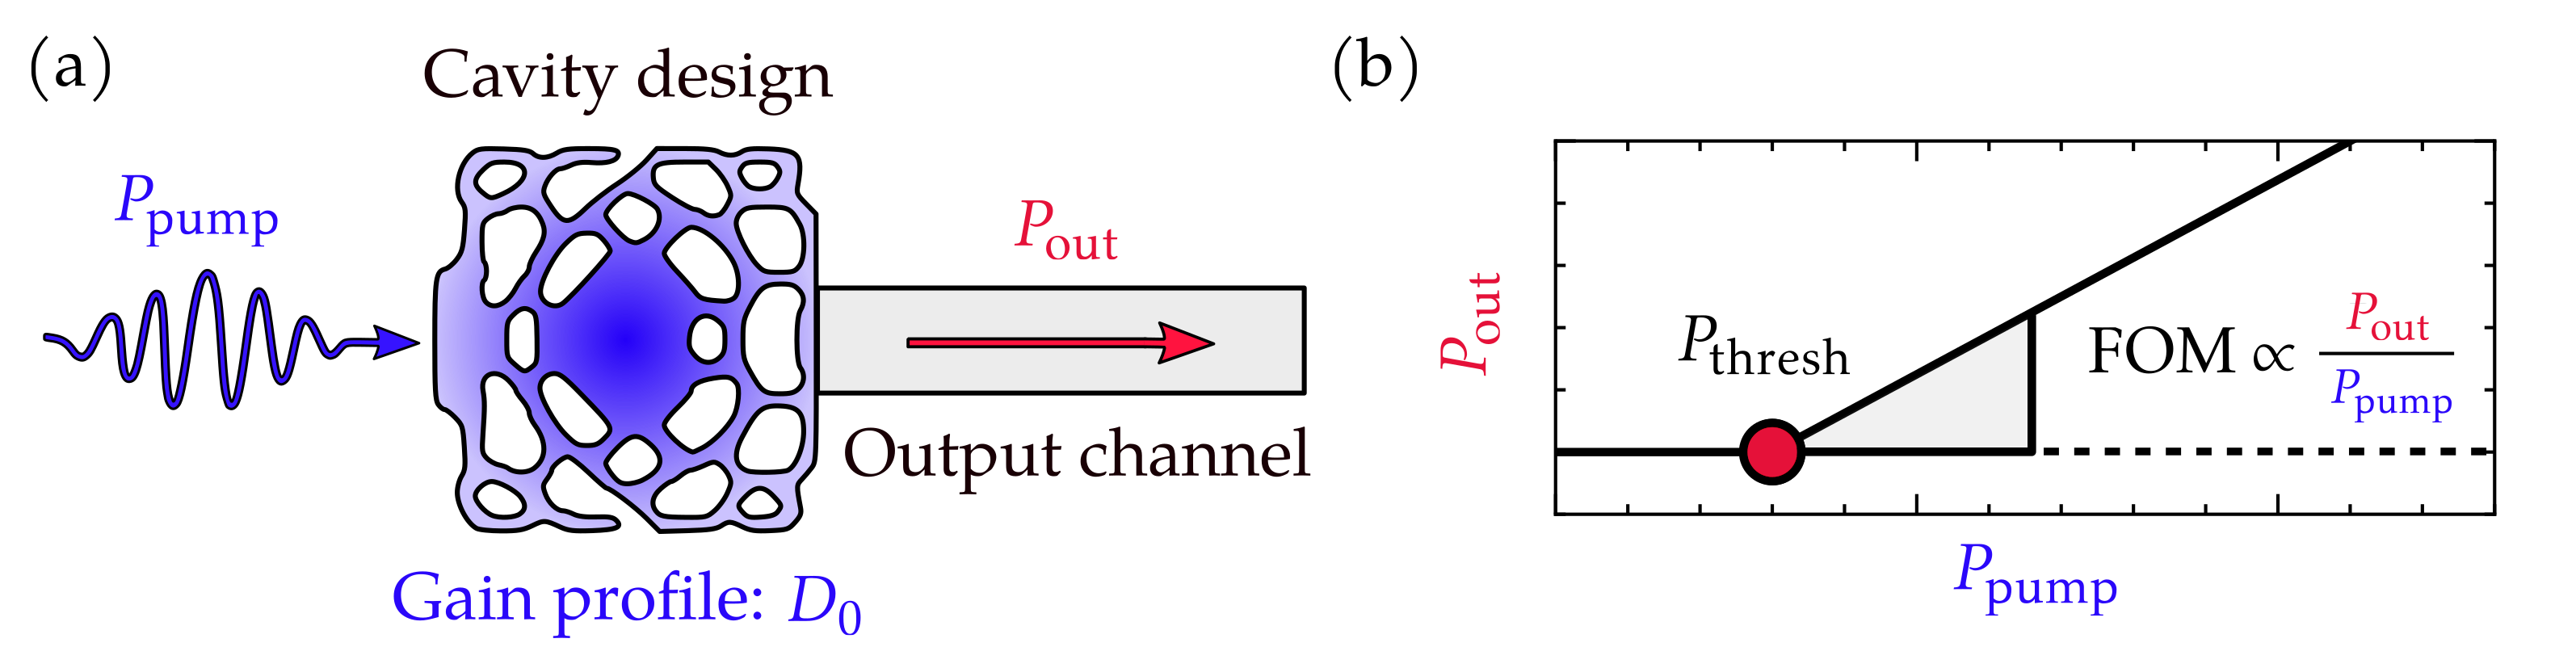
\includegraphics{figures/laser.png}}%%
    \caption{Topology optimization of nanolasers. (a) Working principle of a nanolaser. A pump power ($P_\text{pump}$) excites a a gain medium with profile
    $D_0$ that emits a single lasing mode into an output channel with power $P_\text{out}$. (b) The optimization FOM considers the linear relation between the pump and output power ($P_\text{out}/P_\text{pump}$),
    just above the lasing threshold ($P \gtrapprox P_\text{thres}$). (c) Topology optimization with carrier diffusion effects, where the gain profile $D_0$ is diffused ($\mathbb{S}[D_0]$)
    in the semiconductor-like material. Adapted from~\cite{ownpub4}. MAKE RIGHT PLOT LARGER AND ADJUST THE REST, B SHOULD BE TALLER AND A SHOULD BE SCALED DOWN. FOM SHOULD NOT BE EQUAL.}
    \label{fig:laser2d}
\end{figure}

To circumvent this, in~\cite{ownpub4} we use a synthesis of SPA-SALT, perturbation theory, and coupled mode theory to simplify the problem. 
The two key results of this derivation are the expression of the lasing threshold and the FOM for the optimization that can be evaluated by solving a linear system of equations.
The lasing threshold is given by~\cite{ownpub4} CHANGE GAMMA FACTOR THING
\begin{equation}\label{eq:pump_thresh}
    d_\text{thresh} = \frac{1}{\Gamma Q} = \frac{1}{Q} \frac{\int_{\Omega} \varepsilon_c(\mathbf{r})|\mathbf{E}_{\text{m}}(\mathbf{r})|^2\,  \d \Omega}{\int_{\Omega} D_0(\mathbf{r}) |\mathbf{E}_{\text{m}}(\mathbf{r})|^2\,  \d \Omega}\,.
\end{equation}
where $\mathbf{E}_\text{m}$ is the passive cavity mode, $Q$ is the quality factor of the cavity resonance, and $\Gamma$ is a measure 
of energy confinement in the gain region. From this expression we see that one can reduce the lasing threshold (for more energy-efficient lasers) by increasing $Q$ and decreasing $\Gamma$ by enhancing the energy confinement in the
active medium. Note that in the limit of a single-emitter limit, where $D_0(\mathbf{r})\propto \delta (\mathbf{r}-\mathbf{r^\prime})$ for an emitter located at $\mathbf{r}^\prime$, this expression becomes $d_\text{thresh}=V/Q$, where $V$ is a measure
of the modal volume.

The main result of the work is a FOM that can be evaluated by solving a reciprocal problem where the system is excited from then output port~\cite{ownpub4}
\begin{equation}\label{eq:eff_nl}
    \frac{P_\text{out}}{P_\text{pump}} \propto \frac{\left( \int_{\Omega} D_0(\mathbf{r})|\mathbf{E}_{\text{r}}(\mathbf{r})|^2 \,  \d \Omega \right)^3} {\int_{\Omega} D_0(\mathbf{r}) |\mathbf{E}_{\text{r}}(\mathbf{r})|^4 \,  \d \Omega} = \text{FOM}.
\end{equation}
where $\mathbf{E}_{\text{r}}$ is the field distribution in the reciprocal problem. The FOM is a metric proportional to the laser efficiency ($P_\text{out}/P_\text{pump}$), and is roughly proportional 
to the energy in the cavity ($\sim |\mathbf{E}_{\text{r}}|^6 / |\mathbf{E}_{\text{r}}|^4 \sim |\mathbf{E}_{\text{r}}|^2$), and thus to the $Q$ factor, also contributing to a low
laser threshold (\eqref{eq:pump_thresh}). Thefore, as the optimization progresses the high-$Q$ assumption will become more and more accurate. In the single emitter limit the FOM becomes\footnote{In \cite{ownpub4} we refer to this as the \emph{naive} FOM for nanolaser optimization.}
\begin{equation}\label{eq:SEL}
    \text{FOM}_\text{SEL}=\int_{\Omega} D_0(\mathbf{r}) |\mathbf{E}_{\text{r}}(\mathbf{r})|^2 \d \Omega\,,
\end{equation}
and LDOS-like FOM, which via reciprocity is proportional to the total power emitted into an output channel~\cite[App.~C]{reci}. Note that this FOM is also accurate for a single-point gain region (e.g., a quantum dot),
whose location is randomly distributed in the cavity with a probability density $\sim D_0$. 

\subsection*{Optimization results for extended gain media}

\subsection*{Accounting for gain diffusion}

In semiconductors with extended gain media, it is essential to model the electrical proccess of carrier diffusion. This effect can be introduced by modeling the semiconductor gain medium in the free-carrier approximation\footnote{Neglecting carrier-carrier Coulomb interactions.}, using a difussion 
equation~\cite{csalt}. Using this formalism we derive the same expressions when accounting for carrier diffusion~\cite{ownpub4}, where the lasing threshold is
\begin{equation}\label{eq:pump_thresh_diff}
    d_\text{thresh} = \frac{1}{Q} \frac{\int_{\Omega} \varepsilon_c(\mathbf{r})|\mathbf{E}_{\text{m}}(\mathbf{r})|^2\,  \d \Omega}{\int_{\Omega} \mathbb{S} [D_0] (\mathbf{r}) |\mathbf{E}_{\text{m}}(\mathbf{r})|^2\,  \d \Omega}\,,
\end{equation}
and the FOM is given by
\begin{equation}\label{eq:eff_diff}
    \text{FOM} =  \frac{\left(\int_{\Omega} \mathbb{S} [D_0](\mathbf{r}) |\mathbf{E}_{\text{r}}(\mathbf{r})|^2 \,  \d \Omega\right)^3} {\int_{\Omega} \mathbb{S}\left[ |\mathbf{E}_{\text{r}}|^2\, \mathbb{S} [D_0] \right] (\mathbf{r})|\mathbf{E}_{\text{r}}(\mathbf{r})|^2 \,  \d \Omega}\,.
\end{equation}
These expressions use the diffusion operator $\mathbb{S}^{-1}= \mathbb{I}+\nabla \cdot (R_\nabla^2(\mathbf{r}) \nabla)$, where $\mathbb{I}$ is the identity operator, and $R_\nabla (\mathbf{r})$ is a diffusion lengthscale determined by the spatially- and design-dependent diffusion coefficient combined with the damping/recombination rate. 
In this notation computing $u = \mathbb{S}[b]$ corresponds to solving for the scalar field $u$ in the diffusion problem $\mathbb{S}^{-1}u=b$, where $b$ is a scalar field. 
The difference when accounting for difussion is that now one needs to consider the profile of diffused carriers $\mathbb{S} [D_0]$ in the lasing threshold, and the diffusion of the gain depletion
in the FOM denominator. Note that in the small diffusion limit ($R_\nabla \ll \lambda, \mathbb{S} \approx \mathbb{I}$)
we recover the original expressions in \eqref{eq:pump_thresh} and \eqref{eq:eff_nl}.

Using this new formulation for nanolaser optimization we optimize nanolaser devices in two and three dimensions. In two dimensions we study the effect of the gain region size in 
nanolaser design (Fig. 3 in \cite{ownpub4}), and verify that for point-like gain regions the devices optimizefd for the FOM and an single-emitter limit FOM (\eqref{eq:SEL})
achieve similar performance (limited by the finite size of the tiny gain region), favoring bowtie-like cavity designs
where the in-plane electric field can be concentrated at a bowtie sharpness-limited field singularity. Moreover, we show that for
larger distributed gain media the derived FOM discourages field localization (since $\int \vert \mathbf{E} \vert^2$ is finite), in contrast to the single-emitter limit FOM, 
resulting in a $\approx 3\times$ enhancement when targeting the correct FOM. 

We also see study how accounting for diffusion effects
affects nanolaser designs and performance. As shown in \figref{fig:laser2d}, the device that accounts for diffusion disconnects the cavity from the waveguide while also removing
material from areas of weak electric field, to 
enhance the coupling between the carriers and the optical field, and results in a $\approx 2\times$ enhancement when considering the diffusion-corrected FOM. 

\subsection*{Towards realizable nanolasers: three-dimensional designs}

Finally, we also apply the formalism to design three-dimensional silicon-on-insulator nanolasers (\figref{fig:laser3d}), 
and verify that similar to the two-dimensional case, the FOM discourages field localization while still efficiently coupling to the output waveguide, yielding a $\approx 1.6\times$
enhancement when considering the correct FOM for extended gain media. Note that the enhacement drop with respect to the two-dimensional optimization results
is attributed to the fact that localizing a high-$Q$ resonance is more difficult in three-dimensions.

\begin{figure}[tb]
    \centering
    \makebox[\textwidth][c]{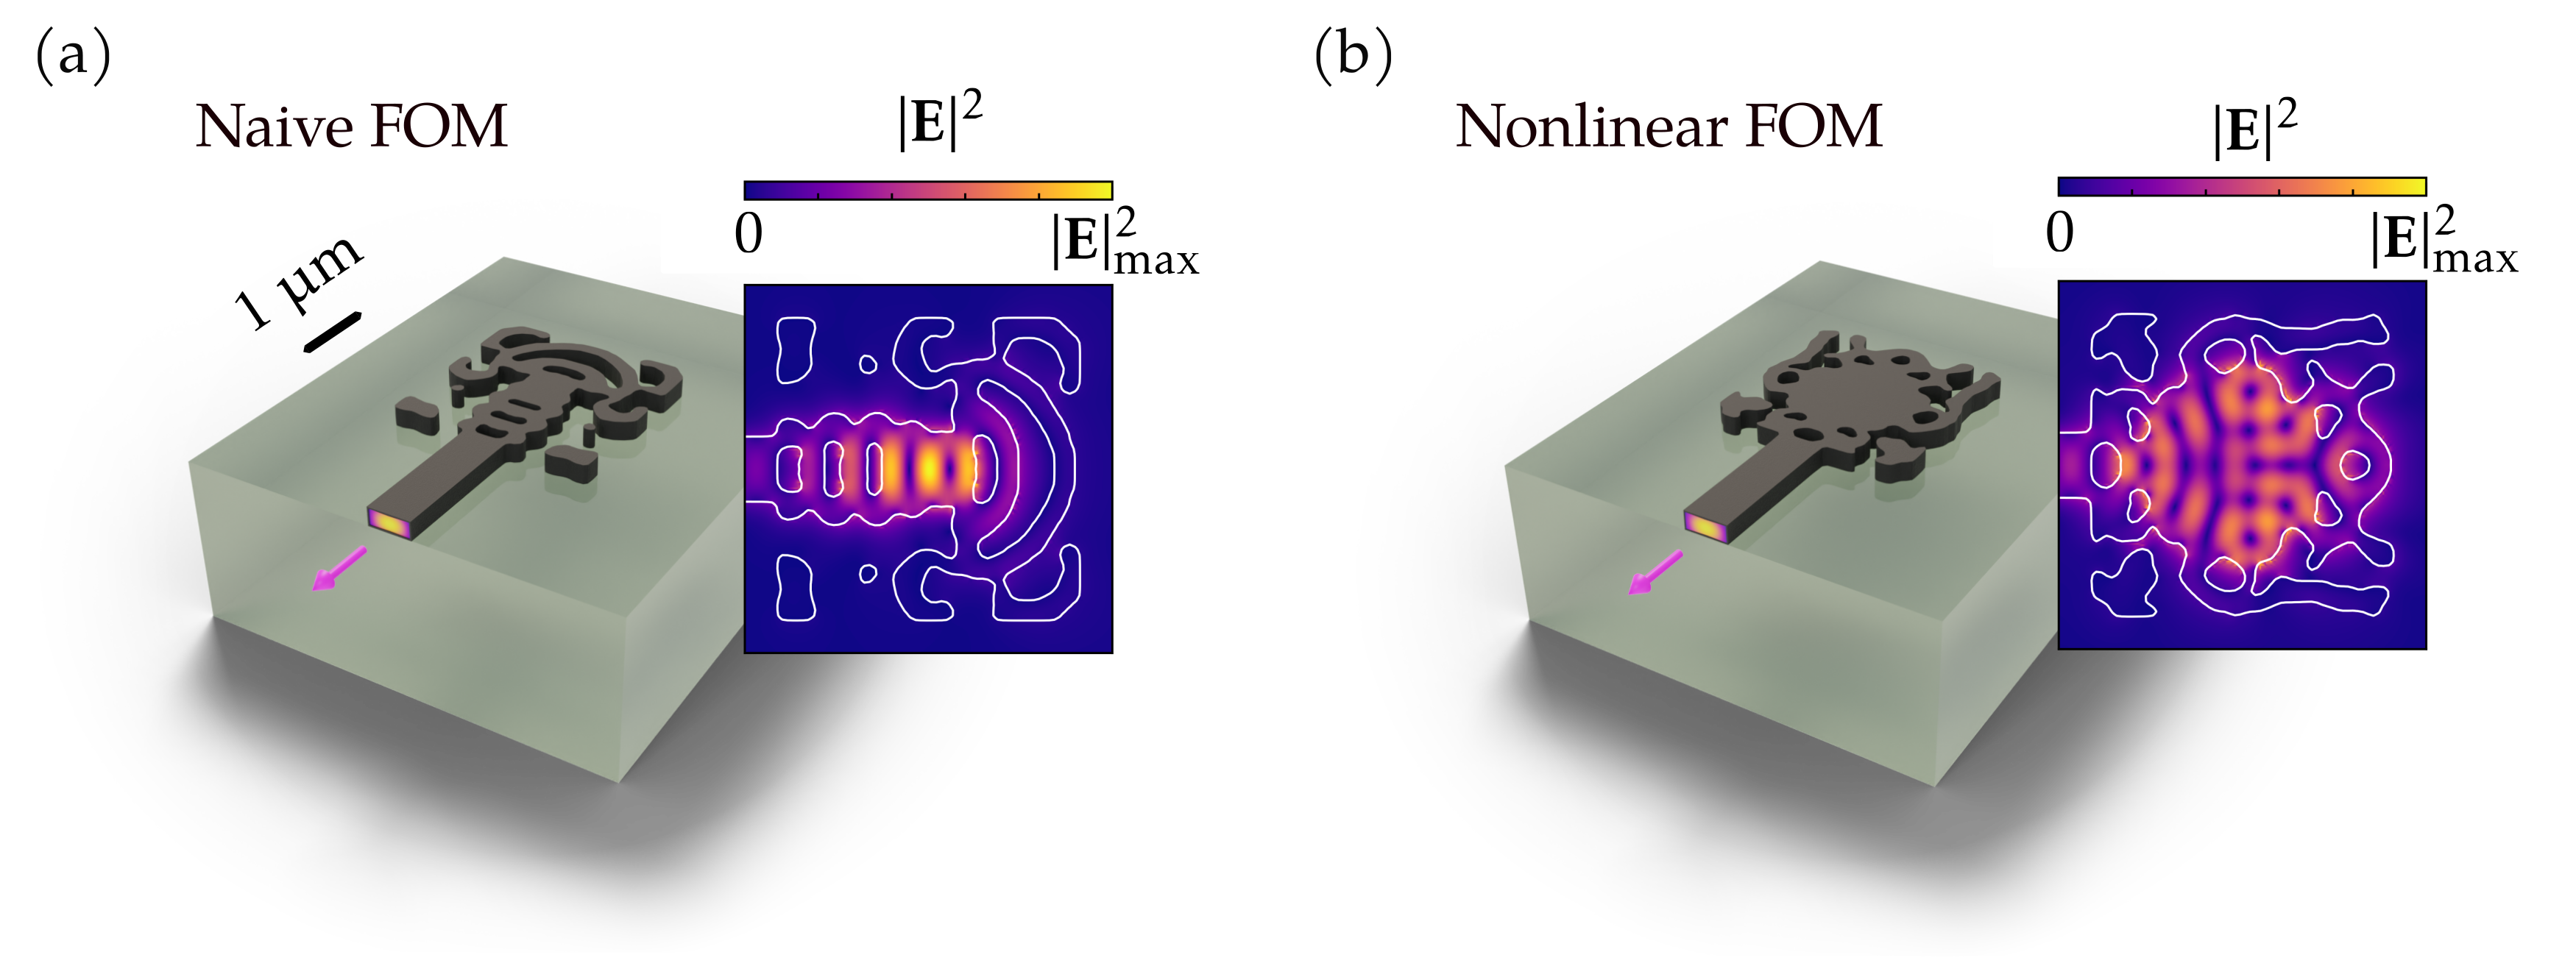
\includegraphics{figures/laser_2.png}}%%
    \caption{Topology-optimized nanolasers in three dimensions. The devices las into the cavity mode (inset plot) and out-couple to the
    mostly-$H_z$ waveguide mode. (a) Device optimized for the naive FOM. (b) Device optimized for the nonlinear FOM.}
    \label{fig:laser3d}
\end{figure}

\subsection*{Outlook and future work}

In conclusion, in \cite{ownpub4} we show that by exploiting perturbative analysis valid in high-$Q$ cavities, one can derive  
an efficient figure of merit (FOM) for laser efficiency that captures resonant enhancement,  
spatial hole-burning, and gain diffusion at little extra computational cost. The FOM evaluation requires only a  
single linear reciprocal Maxwell solve (plus potentially two scalar solves for gain diffusion), making it 
an efficient formulation for laser optimization. This first-principles approach supports inverse nanolaser design and  
future refinements, including accounting for the laser linewidth~\cite{pick}, or (more) accurate pumping models, where optical or electrical pumping could be explicitly
modeled.
